\documentclass[a4paper,12pt]{article}
\usepackage[indonesian]{babel}
\usepackage{graphicx}
\usepackage{multirow}
\usepackage{enumitem}
\usepackage{listings}
\usepackage{wrapfig}
\usepackage[T1]{fontenc}
\usepackage{inconsolata}
\usepackage{lipsum}
\usepackage{adjustbox}
\usepackage{upquote}


\usepackage{color}
\usepackage[table]{xcolor}
\definecolor{lightgray}{rgb}{0.95, 0.95, 0.95}
\definecolor{darkgray}{rgb}{0.4, 0.4, 0.4}
%\definecolor{purple}{rgb}{0.65, 0.12, 0.82}
\definecolor{editorGray}{rgb}{0.95, 0.95, 0.95}
\definecolor{editorOcher}{rgb}{1, 0.5, 0} % #FF7F00 -> rgb(239, 169, 0)
\definecolor{editorGreen}{rgb}{0, 0.5, 0} % #007C00 -> rgb(0, 124, 0)
\definecolor{orange}{rgb}{1,0.45,0.13}		
\definecolor{olive}{rgb}{0.17,0.59,0.20}
\definecolor{brown}{rgb}{0.69,0.31,0.31}
\definecolor{purple}{rgb}{0.38,0.18,0.81}
\definecolor{lightblue}{rgb}{0.1,0.57,0.7}
\definecolor{lightred}{rgb}{1,0.4,0.5}
% CSS
\lstdefinelanguage{CSS}{
  keywords={color,background-image:,margin,padding,font,weight,display,position,top,left,right,bottom,list,style,border,size,white,space,min,width, transition:, transform:, transition-property, transition-duration, transition-timing-function},	
  sensitive=true,
  morecomment=[l]{//},
  morecomment=[s]{/*}{*/},
  morestring=[b]',
  morestring=[b]",
  alsoletter={:},
  alsodigit={-}
}

% JavaScript
\lstdefinelanguage{JavaScript}{
  morekeywords={typeof, new, true, false, catch, function, return, null, catch, switch, var, if, in, while, do, else, case, break},
  morecomment=[s]{/*}{*/},
  morecomment=[l]//,
  morestring=[b]",
  morestring=[b]'
}

\lstdefinelanguage{HTML5}{
  language=html,
  sensitive=true,	
  alsoletter={<>=-},	
  morecomment=[s]{<!-}{-->},
  tag=[s],
  otherkeywords={
  % General
  >,
  % Standard tags
	<!DOCTYPE,
  </html, <html, <head, <title, </title, <style, </style, <link, </head, <meta, />,
	% body
	</body, <body,
	% Divs
	</div, <div, </div>, 
	% Paragraphs
	</p, <p, </p>,
	% scripts
	</script, <script,
  % More tags...
  <canvas, /canvas>, <svg, <rect, <animateTransform, </rect>, </svg>, <video, <source, <iframe, </iframe>, </video>, <image, </image>, <header, </header, <article, </article
  },
  ndkeywords={
  % General
  =,
  % HTML attributes
  charset=, src=, id=, width=, height=, style=, type=, rel=, href=,
  % SVG attributes
  fill=, attributeName=, begin=, dur=, from=, to=, poster=, controls=, x=, y=, repeatCount=, xlink:href=,
  % properties
  margin:, padding:, background-image:, border:, top:, left:, position:, width:, height:, margin-top:, margin-bottom:, font-size:, line-height:,
	% CSS3 properties
  transform:, -moz-transform:, -webkit-transform:,
  animation:, -webkit-animation:,
  transition:,  transition-duration:, transition-property:, transition-timing-function:,
  }
}

\lstdefinestyle{htmlcssjs} {%
  % General design
%  backgroundcolor=\color{editorGray},
  basicstyle={\footnotesize\ttfamily},   
  frame=single,
  % line-numbers
  % Code design
  identifierstyle=\color{black},
  keywordstyle=\color{blue}\bfseries,
  ndkeywordstyle=\color{editorGreen}\bfseries,
  stringstyle=\color{editorOcher}\ttfamily,
  commentstyle=\color{brown}\ttfamily,
  % Code
  language=HTML5,
  alsolanguage=JavaScript,
  alsodigit={.:;},	
  tabsize=2,
  showtabs=false,
  showspaces=false,
  showstringspaces=false,
  extendedchars=true,
  breaklines=true,
  % German umlauts
  literate=%
  {Ö}{{\"O}}1
  {Ä}{{\"A}}1
  {Ü}{{\"U}}1
  {ß}{{\ss}}1
  {ü}{{\"u}}1
  {ä}{{\"a}}1
  {ö}{{\"o}}1
}
%
\lstdefinestyle{py} {%
language=python,
literate=%
*{0}{{{\color{lightred}0}}}1
{1}{{{\color{lightred}1}}}1
{2}{{{\color{lightred}2}}}1
{3}{{{\color{lightred}3}}}1
{4}{{{\color{lightred}4}}}1
{5}{{{\color{lightred}5}}}1
{6}{{{\color{lightred}6}}}1
{7}{{{\color{lightred}7}}}1
{8}{{{\color{lightred}8}}}1
{9}{{{\color{lightred}9}}}1,
basicstyle=\footnotesize\ttfamily, % Standardschrift
numbers=left,               % Ort der Zeilennummern
%numberstyle=\tiny,          % Stil der Zeilennummern
%stepnumber=2,               % Abstand zwischen den Zeilennummern
numbersep=5pt,              % Abstand der Nummern zum Text
tabsize=4,                  % Groesse von Tabs
extendedchars=true,         %
breaklines=true,            % Zeilen werden Umgebrochen
keywordstyle=\color{blue}\bfseries,
frame=b,
commentstyle=\color{brown}\itshape,
stringstyle=\color{editorOcher}\ttfamily, % Farbe der String
showspaces=false,           % Leerzeichen anzeigen ?
showtabs=false,             % Tabs anzeigen ?
xleftmargin=17pt,
framexleftmargin=17pt,
framexrightmargin=5pt,
framexbottommargin=4pt,
%backgroundcolor=\color{lightgray},
showstringspaces=false,      % Leerzeichen in Strings anzeigen ?
}%
%
\definecolor{dkgreen}{rgb}{0,.6,0}
\definecolor{dkblue}{rgb}{0,0,.6}
\definecolor{dkyellow}{cmyk}{0,0,.8,.3}

\lstdefinestyle{PHP}{
  language        = php,
  basicstyle      = \small\ttfamily,
  keywordstyle    = \color{dkblue},
  stringstyle     = \color{red},
  identifierstyle = \color{dkgreen},
  commentstyle    = \color{gray},
  emph            =[1]{php},
  emphstyle       =[1]\color{black},
  emph            =[2]{if,and,or,else},
  emphstyle       =[2]\color{dkyellow}}
\lstset{
    showstringspaces=false,
    frame=single,
    breaklines=true,
    rulecolor=\color{black}
}
%

\graphicspath{ {./img/} }
\begin{document}
\title{ {\Large Laporan Praktikum}\\ Pemrograman Web Client\\{\Large Pertemuan 5}}

\author{Aldzikri Dwijayanto Prathama 
	\\195410189
	\\Informatika}
\makeatletter
\begin{titlepage}
	\begin{center}
		{\huge \bfseries \@title }\\[14ex]
		
\includegraphics[scale=.8]{logo}\\[4ex]
		{\large \@author}\\[12ex]
		{\large \bfseries {SEKOLAH TINGGI MANAJEMEN INFORMATIKA DAN KOMPUTER
				AKAKOM YOGYAKARTA}}
	\end{center}


%{\large \@date} 
\end{titlepage}
\makeatother
%\maketitle
\newpage
\tableofcontents
\newpage
\section{Tujuan}
\begin{enumerate}
    \item Menuliskan script kontainer form beserta atributnya
    \item Menuliskan element input teks dan submit
    \item Menyiapkan server web
    \item Menguji input form dengan mengirim data ke server dan menampilkan data dari server
    \item Menjelaskan perbedaan metode POST dan GET
\end{enumerate}
\section{Dasar Teori}
Form atau formulir adalah media untuk menerima input dari user, contohnya saat
proses login untuk memasukkan user name dan password. Data-data yang diinputkan
melalui form akan dikirim ke server, bianya diikuti dengan proses penyimpanan di
database. Contoh saat mendaftar di email.
Tag yang digunakan adalah <form>, terdapat beberapa atribut yang sering dipakai
terkait dengan proses pengiriman data ke server, yaitu:
\begin{enumerate}
    \item Action: mengatir URL kemana data akan dikirim.
    \item method: cara protokol http mengirim data, terdapat 2 cara yaitu POST dan GET
    \item target: menentukan lokasi yang digunakan untuk menampilkan respon dari
data yang telah diterima server setelah proses submit. Pilihan target yaitu: \_blank,
\_self, \_parent, \_top
\end{enumerate}
Perbedaan pengiriman data dengan method POST atau GET dapat dilihat pada URL
website. Jika menggunakan method GET maka data yang dikirim akan terlihat sedangkan
dengan method POST datanya tidak akan terlihat.

\newpage

\section{Pembahasan}
\subsection{Praktik}
Pertama jalankan Apache, MySQL, dan PHP terlebih dahulu.
\begin{center}
    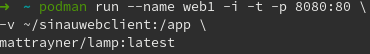
\includegraphics[scale=.8]{1.png}\\[4ex]
    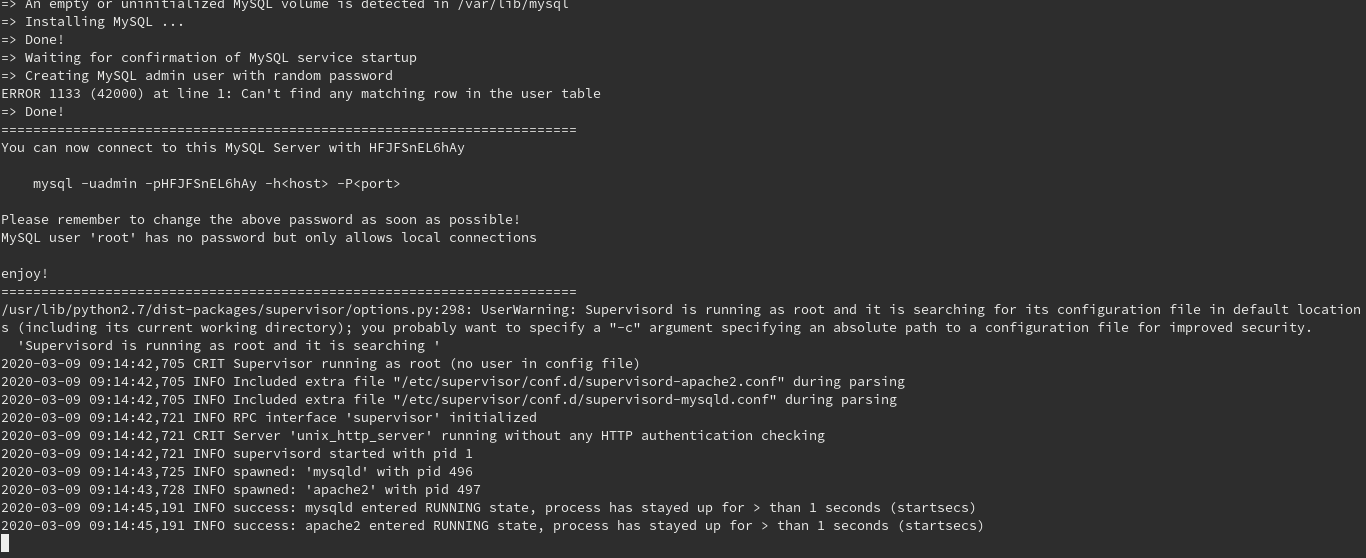
\includegraphics[width=\linewidth]{2.png} 
\end{center}
Kemudian ketik CSS berikut kemudian simpan didalam folder css, dan beri nama style.css.
\begin{lstlisting}[style=htmlcssjs]
.container {
    width: 50%;
    margin: 0 auto;
}
span {
    display: block;
    margin-bottom: 20px;
}
.success {
    display: block;
    margin-top: 20px;
    margin-bottom: 0;
    font-size: 14px;
}
b {
    color: green;
}


div.main{
    width: 306px;
    padding: 10px 50px 30px;
    border: 2px solid gray;
    float: left;
    margin-top: 15px;
}
input[type=text]{
    width: 96%;
    height: 25px;
    border: 1px solid;
}
\end{lstlisting}
\newline
file css tersebut akan mengatur element dan mendeklarasikan class yang ditulis. Class container akan mengatur elemen dengan luas menjadi 50\%, dan margin yang diatur otomatis.
Elemen span displaynya diatur menjadi block, dan ukuran margin bawahnya diatur sebesar 20px.
Class success akan mengatur display menjadi block, mengatur margin atas sebesar 20px, margin bawah sebesar 0, dan mengatur besar font sebesar 14px.
Lalu tag b akan diatur wawrnanya menjadi hijau.
div.main diatur lebarnya sebesar 206px, padding mmenjadi 10px 50px 30px, dan float ke kiri, sedangkan margin atas diatur sebesar 15px.
Untuk kolom input diatur lebarnya menjadi 96\%, tingginya 25px, dan bordernya berukuran 1px dan modelnya solid.\\[2ex]

Lalu buat skrip php yang bertugas untuk mengolah data, file tersebut kita beri nama proses.php.
\begin{lstlisting}[style=PHP]
<?php
if (isset($_POST['fnama'])) {
    $fnama = $_POST['fnama'];
    $lalamat = $_POST['lalamat'];
    echo "<span class='success'>Dengan <b>METODE POST</b></span><br/>";
    echo "Nama : " . $fnama . "<br/>Alamat : " . $lalamat;
}
//------------------------------------------------------
if (isset($_GET['fnama'])) {
    $fnama = $_GET['fnama'];
    $lalamat = $_GET['lalamat'];
    echo "<span class='success'>Dengan <b>METODE GET</b></span><br/>";
    echo "Nama : " . $fnama . "<br/>Alamat : " . $lalamat;
}
?>
\end{lstlisting}
Script PHP tersebut akan mengambil input dari user, dan memasukkannya ke variabel. Selain itu terdapat pemilihan, jika method menggunakan POST, akan mengeprint Dengan METODE POST, sedangkan jika menggunakan method GET, maka akan mengeprint Dengan METODE GET.\\[2ex]

Selanjutnya buat file dengan nama index.php, lalu ketik seperti berikut.
\begin{lstlisting}[style=PHP]
<!DOCTYPE html>
<html>

<head>
    <link rel="stylesheet" href="css/style.css" />
</head>

<body>
    <div class="container">
        <div class="main">
            <form method="get" action="index.php" id="form">
                <h2>DATA IDENTITAS</h2>
                <hr />
                <label>Nama :</label>
                <input type="text" name="fnama" id="fnama" />
                <label>Alamat :</label>
                <input type="text" name="lalamat" id="lalamat" />
                <input type="submit" name="submit" id="submit" value="submit">
            </form>
            <?php include "proses.php"; ?>
        </div>
    </div>
</body>

</html>
\end{lstlisting}
File php tersebut berfungsi sebagai halaman utama. Selain itu terdapat juga form yang berfungsi untuk menerima input dari user. Setelah user memasukkan data ke form, maka file php
ini akan memanggil file proses.php yang akan memproses data yang sudah dimasukkan.\\[2ex]

Jika kita membuka file index.php melalui web server, dan memasukkan data ke form, maka tampilannya seprti berikut
\begin{center}
    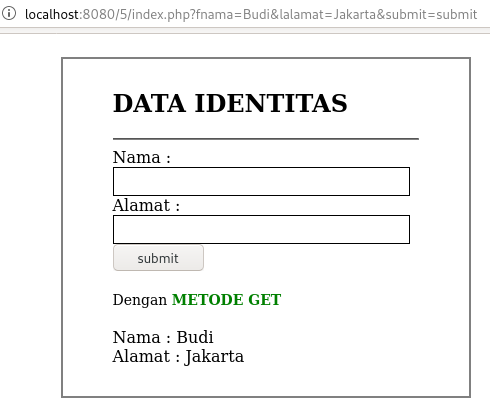
\includegraphics[scale=.6]{3.png} 
\end{center}
Pada url bar terlihat, setelah kita memasukkan data, dan menklik submit, data yang sudah kita masukkan akan muncul pada url bar. Dan karena proses.php, setelah data dimasukkan
dibawah form akan muncul method apa yang digunakan untuk mengirim data, dan mengeprint data yang kita masukkan.\\[2ex]

Selanjutnya kita rubah file index.php pada baris berikut
\begin{lstlisting}[style=PHP]
<form method="get" action="index.php" id="form">
\end{lstlisting}
Method dirubah menjadi POST seperti berikut
\begin{lstlisting}[style=PHP]
<form method="post" action="index.php" id="form">
\end{lstlisting}

Setelah kita rubah dan simpan lalu buka di browser dan isikan data.
\begin{center}
    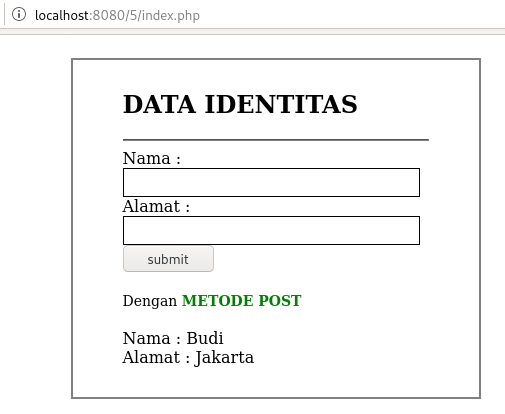
\includegraphics[scale=.6]{4.png} 
\end{center}
Setelah method dirubah menjadi post, hasilnya sedikit berbeda dengan sebelumnya. Jika method menggunakan get, data yang dimasukkan tidak muncul pada urlbar.

\newpage

\subsection{Latihan}
Pada latihan, file index.php dirubah untuk menambah isian untuk input bomor hp dan tanggal lahir.\\
\begin{lstlisting}[style=PHP]
<!DOCTYPE html>
<html>

<head>
    <link rel="stylesheet" href="css/style.css" />
</head>

<body>
    <div class="container">
        <div class="main">
            <form method="post" action="index.php" id="form">
                <h2>DATA IDENTITAS</h2>
                <hr />
                <label>Nama :</label>
                <input type="text" name="fnama" id="fnama" />
                <label>Alamat :</label>
                <input type="text" name="lalamat" id="lalamat" />
                <label>No Telp :</label>
                <input type="text" name="telp" id="telp" />
                <label>Tgl Lahir :</label>
                <input type="text" name="lahir" id="lahir" />
                <input type="submit" name="submit" id="submit" value="submit">
            </form>
            <?php include "proses.php"; ?>
        </div>
    </div>
</body>

</html>
\end{lstlisting}
Tambahkan baris dengan struktur yang dengan form sebelumnya, rubah tabel, name dan id.\\
Lalu ubah juga file proses.php.
\begin{lstlisting}[style=PHP]
<?php
if (isset($_POST['fnama'])) {
    $fnama = $_POST['fnama'];
    $lalamat = $_POST['lalamat'];
    $telp = $_POST['telp'];
    $lahir = $_POST['lahir'];
    echo "<span class='success'>Dengan <b>METODE POST</b></span><br/>";
    echo "Nama : " . $fnama . "<br/>Alamat : " . $lalamat . "<br/> No Telp : " . $telp . "<br/> Tgl Lahir : " . $lahir;
}
//------------------------------------------------------
if (isset($_GET['fnama'])) {
    $fnama = $_GET['fnama'];
    $lalamat = $_GET['lalamat'];
    $telp = $_GET['telp'];
    $lahir = $_GET['lahir'];
    echo "<span class='success'>Dengan <b>METODE GET</b></span><br/>";
    echo "Nama : " . $fnama . "<br/>Alamat : " . $lalamat . "<br/> No Telp : " . $telp . "<br/> Tgl Lahir : " . $lahir;
}
?>
\end{lstlisting}
Untuk file proses.php kita tambhkan variabel, dan tambahkan variabel tersebut di echo.\\
Buka di browser dan isi dengan data.
\begin{center}
    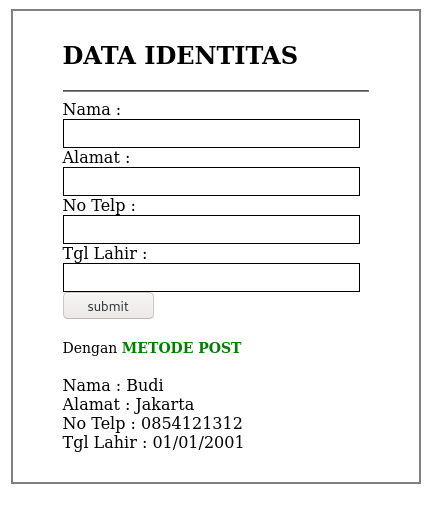
\includegraphics[scale=.6]{5.png} 
\end{center}

\newpage

\subsection{Tugas}
Menyimpan data ke database.\\
Buat database, dan tabel baru menggunakan DBeaver. Lalu buat kolom untuk menyimpan nama, alamat, nomor hp, dan tanggal lahir.
\begin{center}
    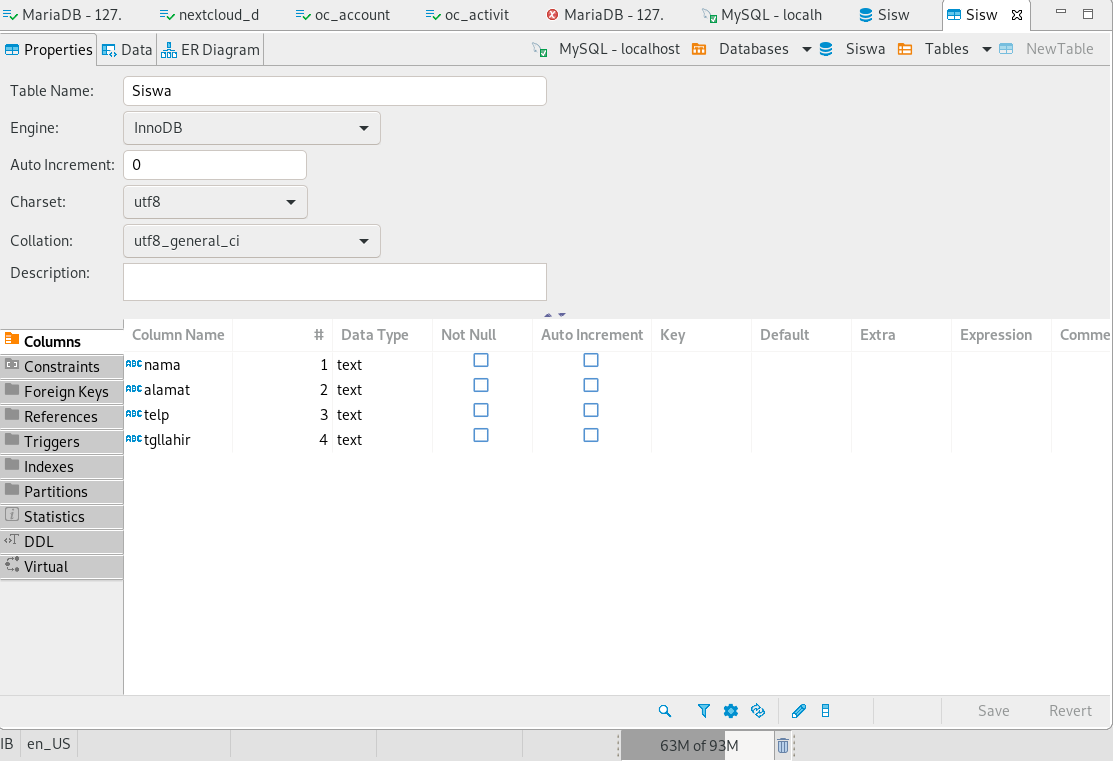
\includegraphics[scale=.4]{6.png} 
\end{center}
Lalu modifikasi file proses.php
\begin{lstlisting}[style=PHP]
<?php
$server="localhost";
$username="admin";
$password="91Eix1bS8iQ4";
$dbname="Data";
$link = mysqli_connect($server, $username,$password,$dbname);
if (!$link) {
      die("Connection failed: " . mysqli_connect_error());
}
echo "Connected to sql";
$fnama = mysqli_real_escape_string($link, $_REQUEST['fnama']);
$lalamat = mysqli_real_escape_string($link, $_REQUEST['lalamat']);
$telp = mysqli_real_escape_string($link, $_REQUEST['telp']);
$lahir = mysqli_real_escape_string($link, $_REQUEST['lahir']);
if (isset($_POST['fnama'])) {
    $fnama = $_POST['fnama'];
    $lalamat = $_POST['lalamat'];
    $telp = $_POST['telp'];
    $lahir = $_POST['lahir'];
    echo "<span class='success'>Dengan <b>METODE POST</b></span><br/>";
    echo "Nama : " . $fnama . "<br/>Alamat : " . $lalamat . "<br/> No Telp : " . $telp . "<br/> Tgl Lahir : " . $lahir;

    $sql = "INSERT INTO Siswa (nama, alamat, telp, tgllahir) VALUES ('$fnama', '$lalamat', '$telp', '$lahir')";
    if (mysqli_query($link, $sql)) {
        echo "<br/>Data berhasil dimasukkan";
    }
    else {
        echo "<br/>Error: " . $sql . "<br>" . mysqli_error($link);
    }
}
//-----------------------------------------------------
if (isset($_GET['fnama'])) {
    $fnama = $_GET['fnama'];
    $lalamat = $_GET['lalamat'];
    $telp = $_GET['telp'];
    $lahir = $_GET['lahir'];
    echo "<span class='success'>Dengan <b>METODE GET</b></span><br/>";
    echo "Nama : " . $fnama . "<br/>Alamat : " . $lalamat . "<br/> No Telp : " . $telp . "<br/> Tgl Lahir : " . $lahir;

    $sql = "INSERT INTO Siswa (nama, alamat, telp, tgllahir) VALUES ('$fnama', '$lalamat', '$telp', '$lahir')";
    if (mysqli_query($link, $sql)) {
        echo "<br/>Data berhasil dimasukkan";
    }
    else {
        echo "<br/>Error: " . $sql . "<br>" . mysqli_error($link);
    }
}
    
mysqli_close($link);

?>
\end{lstlisting}
Setelah itu buka file index.php menggunakan browser, dan isikan data.
\begin{center}
    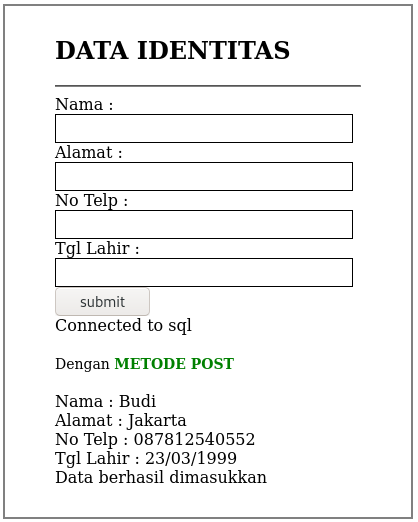
\includegraphics[scale=.6]{7.png} 
\end{center}
Jika data berhasil dimasukkan ke MySQL maka data akan terlihat di tabel pada aplikasi DBeaver.
\begin{center}
    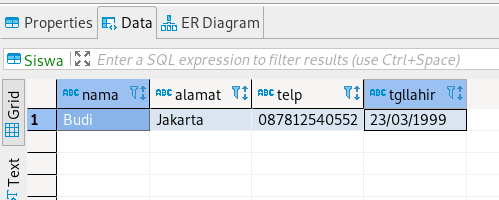
\includegraphics[scale=.6]{8.png} 
\end{center}

\newpage

\section{Kesimpulan}
Setelah praktik ini, mahasiswa mampu menuliskan script kontainer form beserta atributnya, menuliskan element input teks dan submit, menyiapkan server web, menguji input form dengan mengirim data ke server dan menampilkan data dari server, dan menjelaskan perbedaan metode POST dan GET



\end{document}
